\documentclass[report.tex]{subfiles}
\begin{document}

\chapter{Excercise 1A: single mass}

\begin{figure}[H]
  \centering
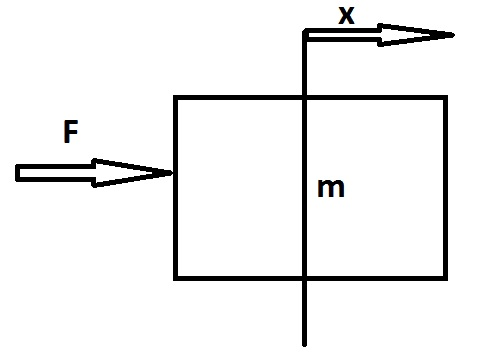
\includegraphics[width=0.5\textwidth,height=\textheight,keepaspectratio]{1A3_system}
\caption{Bode plot of the single mass system}
\label{fig:1A3_system}
\end{figure}

The single mass system is shown as free body diagram in figure~\ref{fig:1A3_system}. The idea is to analyze the dynamic behavior of this mass and then design a controller which can control the system matching a few design criteria. In the following analysis the differences in behavior caused by the variation of the parameters are observed. Specified properties are: 
$ m = 0.1 $

The frequency plot given by diet is shown in figure ~\ref{fig:1A3a_bode}.
From this plot it can be concluded that the gain 1 frequency is: $0.5Hz$

\begin{figure}[H]
  \centering
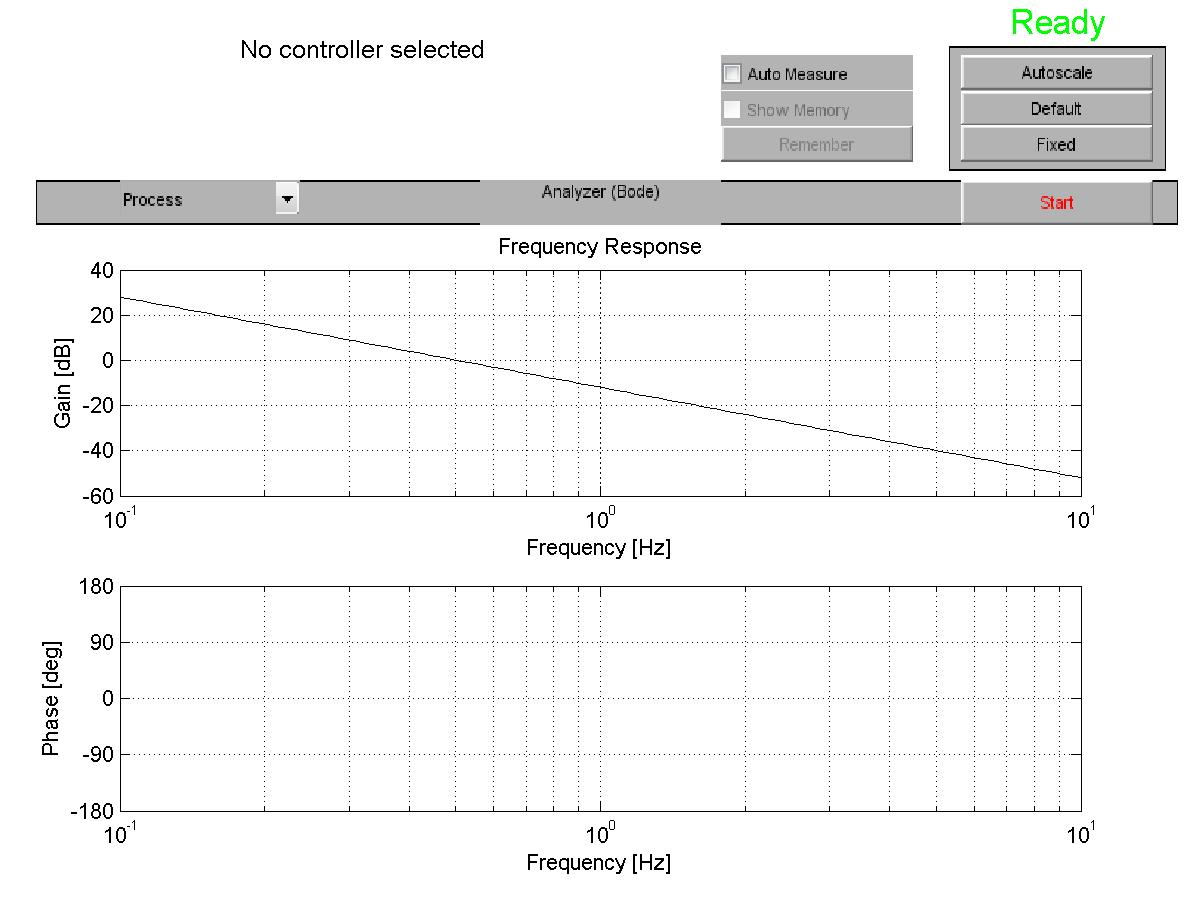
\includegraphics[width=\textwidth,height=\textheight,keepaspectratio]{1A3a_bode}
\caption{Bode plot of the single mass system}
\label{fig:1A3a_bode}
\end{figure}


The differential equation for this systems is defined as

\begin{equation}
\label{eq:ex1a_diff}
m\ddot{x} = F
\end{equation}

This results in a transfer function by combining following equation
\begin{equation}
\label{eq:ex1a_tf_mass_2}
mX(S)s^2 = F(s) => H(S) = \frac{X(S)}{F(S)} = \frac{1}{ms^2}
\end{equation}

To determine the frequency where the gain is 1 equation~\ref{eq:ex1a_tf_freq_1} needs to be solved. 
\begin{equation}
\label{eq:ex1a_tf_freq_1}
|H(jw)| = |\frac{1}{m(j\omega)^2}| = \frac{1}{m\omega^2} = 1
\end{equation}

The following frequency will be:
\begin{equation}
\label{eq:ex1a_tf_freq_2}
\omega = 2\pi f = sqrt(\frac{1}{m}) => f = \frac{1}{2\pi}sqrt(\frac{1}{m}) 
\end{equation}

This system needs to be stabilized. For this a controller with the form $C(s) = k_p + k_v s$ is used.

The step responses below shows one the following things: 
\begin{itemize}
\item{It can be seen that an higher $k_p$ causes an higher overshoot and a little oscillation, but at the same time a faster rise time and settling time. This can be seen when figure~\ref{fig:1A4_time} and figure ~\ref{fig:1A4_time_k}}
\item{A higher $k_v$ on the other hand causes no overshoot and a very vast rise and settling time, as can be seen when figure~\ref{fig:1A4_time} and figure ~\ref{fig:1A4_time_v} are compared. So higher $k_v$ particularly increases the speed of the system, without having the drawbacks of an big overshoot} 
\end{itemize}

\begin{figure}
  \centering
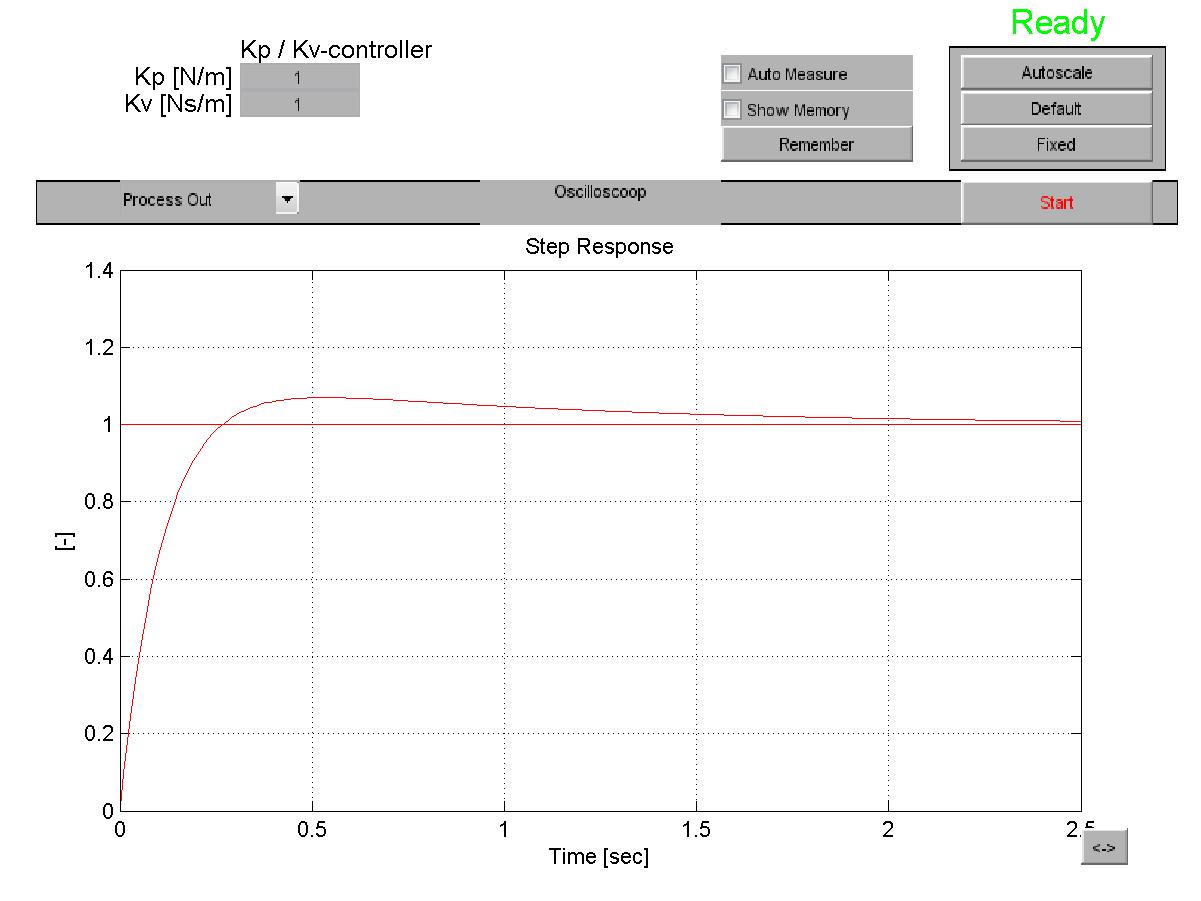
\includegraphics[width=\textwidth,height=\textheight,keepaspectratio]{1A4_time}
\caption{Step response plot of the single mass system with controller $C(S)$ with  $k_p = 1, k_v = 1$}
\label{fig:1A4_time}
\end{figure}

\begin{figure}
  \centering
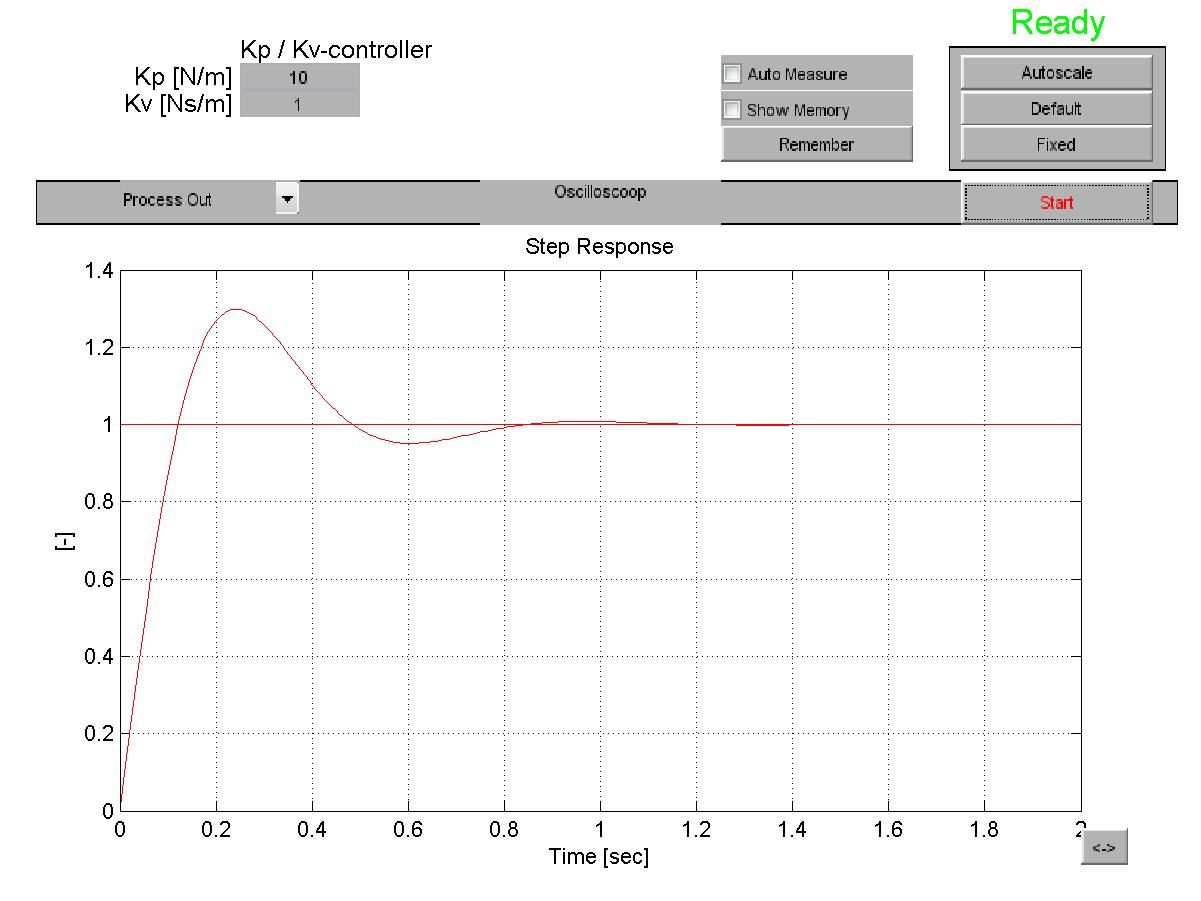
\includegraphics[width=\textwidth,height=\textheight,keepaspectratio]{1A4_time_k}
\caption{Step response plot of the single mass system with controller $C(S)$ with  $k_p = 10, k_v = 1$}
\label{fig:1A4_time_k}
\end{figure}

\begin{figure}[H]
  \centering
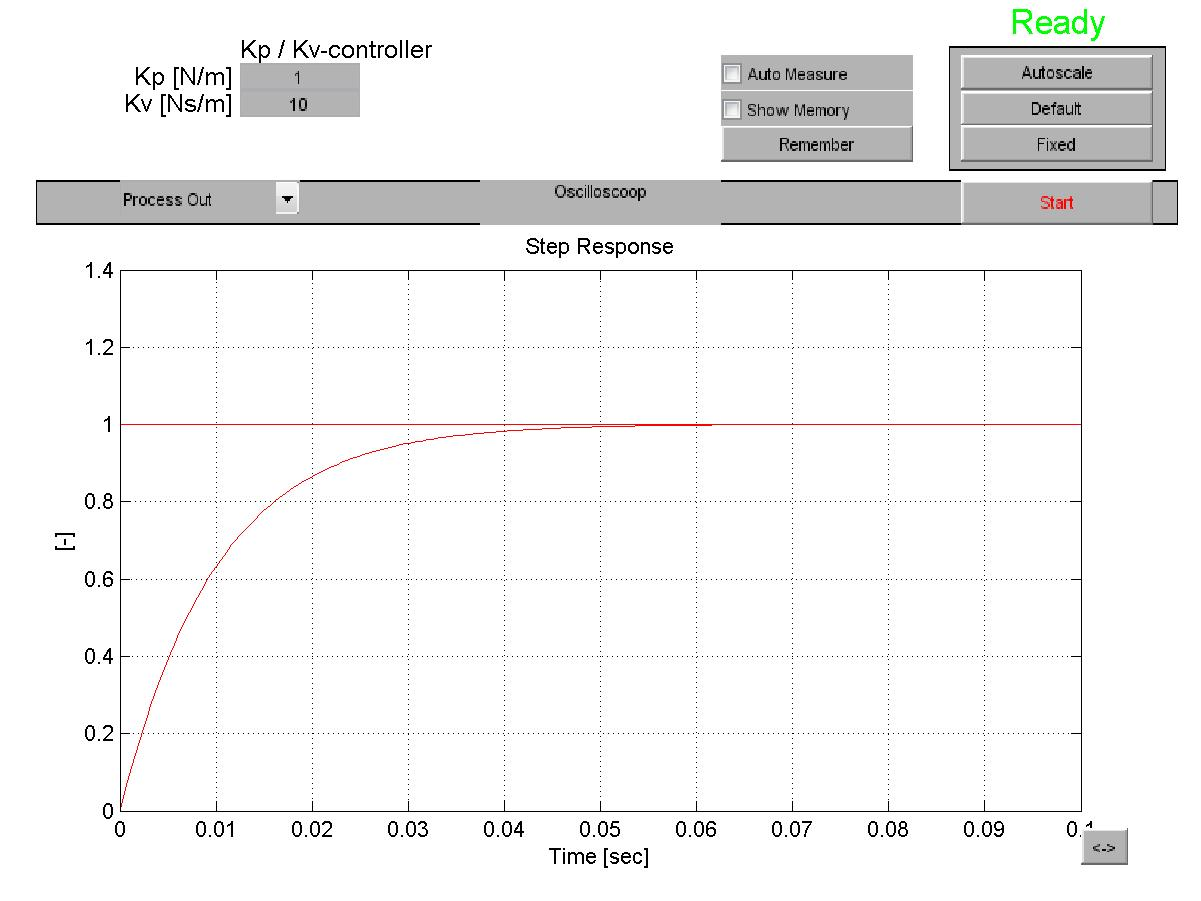
\includegraphics[width=\textwidth,height=\textheight,keepaspectratio]{1A4_time_v}
\caption{Step response plot of the single mass system with controller $C(S)$ with  $k_p = 1, k_v = 10$}
\label{fig:1A4_time_v}
\end{figure}

The resulting bode plot is showed in figure~\ref{fig:1A4_bode}

\begin{figure}
  \centering
    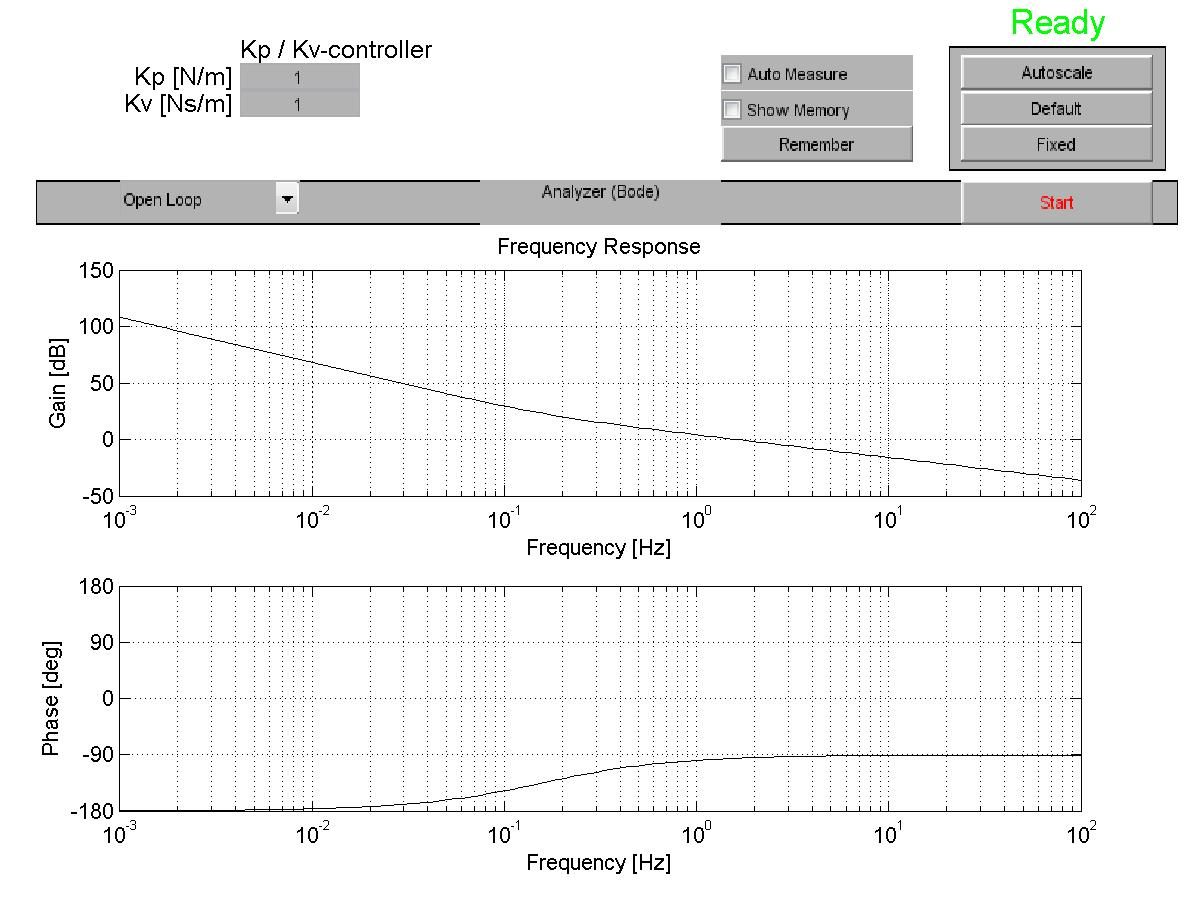
\includegraphics[width=\textwidth,height=\textheight,keepaspectratio]{1A4_bode}
 	\caption{Bode plot of the single mass system with controller $C(S)$}
  \label{fig:1A4_bode}
\end{figure}
\newpage
To investigate the effect of varying the controller parameters $K_p$ and $K_v$ another 2 bode plots, figure figure~\ref{fig:1A4_bode_k} and figure~\ref{fig:1A4_bode_v}, have been created. 
\begin{figure}
  \centering
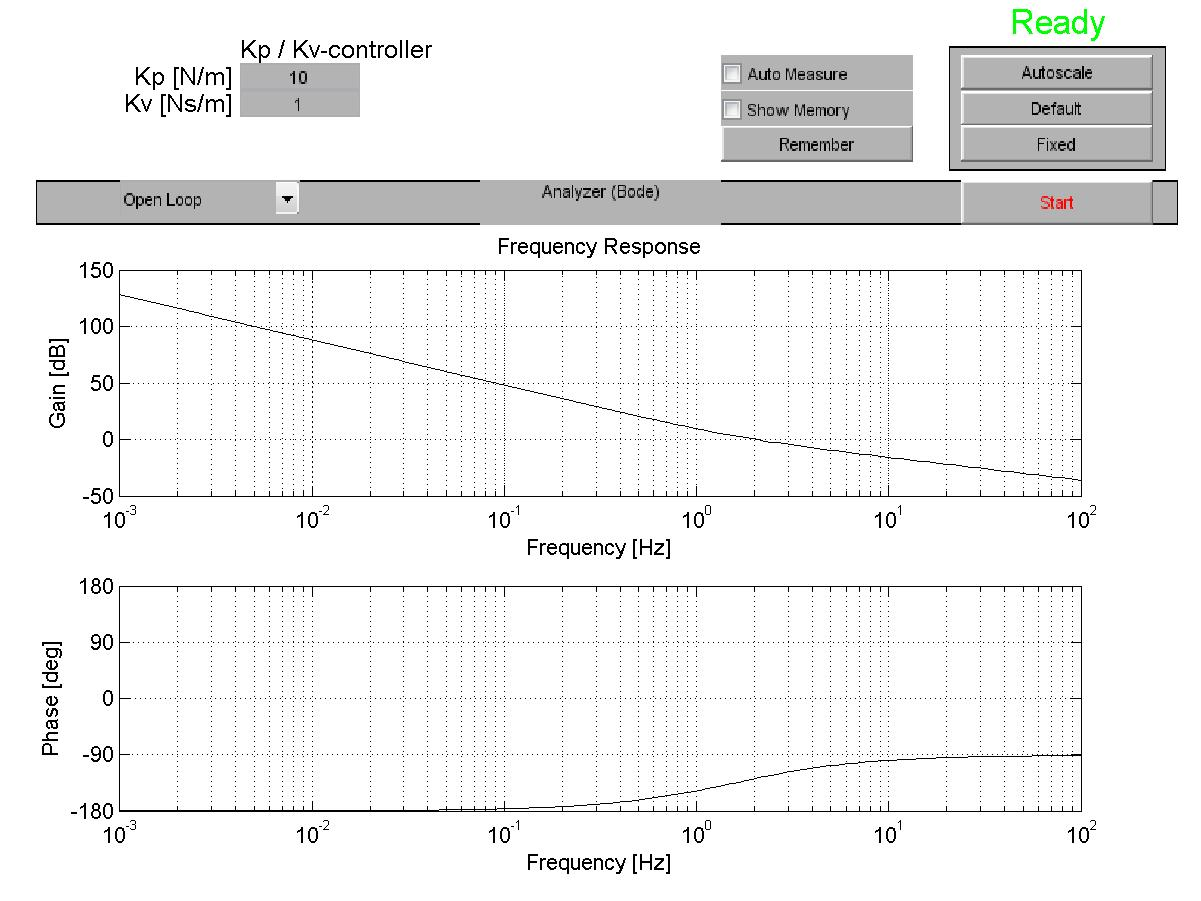
\includegraphics[width=\textwidth,height=\textheight,keepaspectratio]{1A4_bode_k}
\caption{Bode plot of the single mass system with controller $C(S)$ with higher $k_p = 10, k_v
 = 1$}
\label{fig:1A4_bode_k}
\end{figure}

\begin{figure}
  \centering
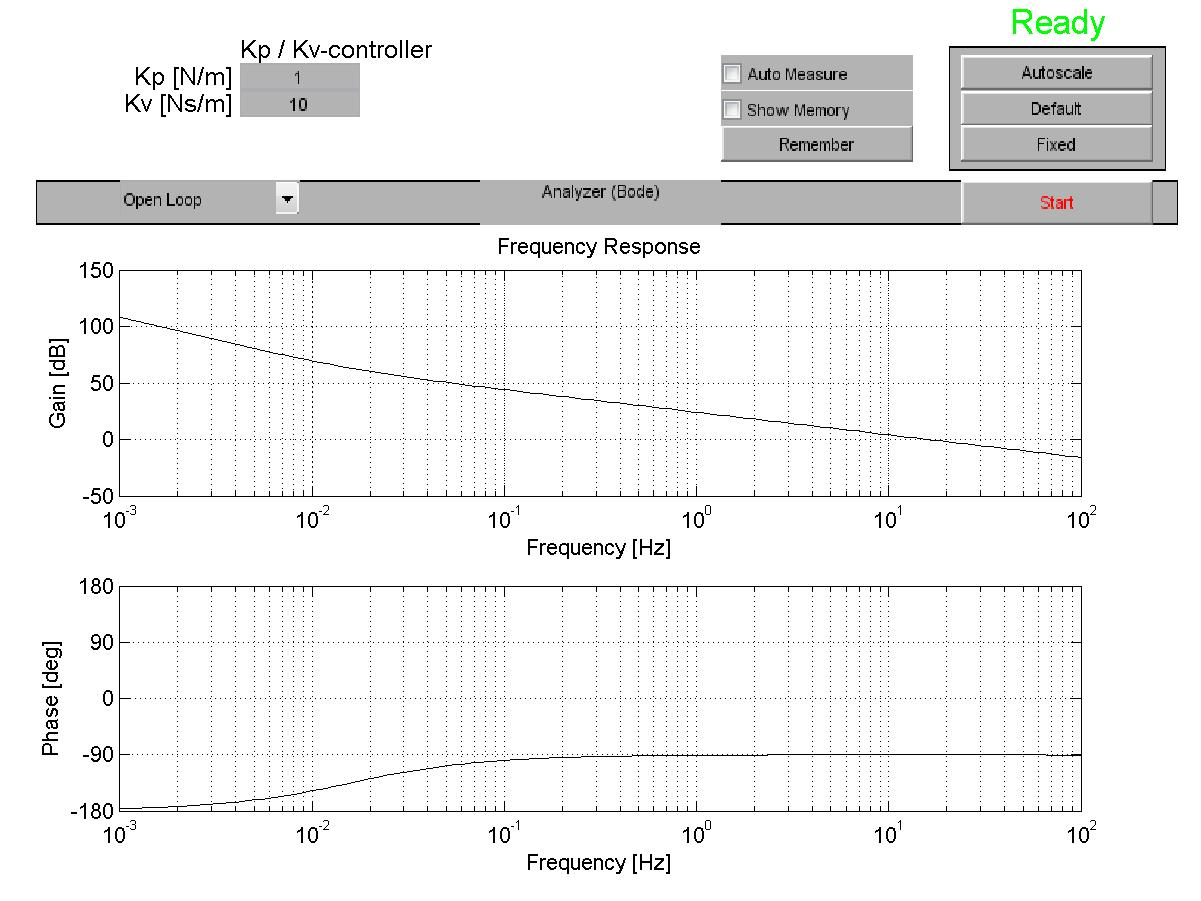
\includegraphics[width=\textwidth,height=\textheight,keepaspectratio]{1A4_bode_v}
\caption{Bode plot of the single mass system with controller $C(S)$ with higher $k_p = 1, k_v = 10$}
\label{fig:1A4_bode_v}
\end{figure}

The following effects on the bode plots can be observed:
\begin{itemize}
\item{The effect of the zero moves with higher $k_p$ to higher frequencies. This can be seen at the buckle from $-40 dB$ to $-20 dB$ that is moved from somewhere around $0.5 Hz$ to $5 Hz$}
\item{The total gain of increases with higher $k_p$. You can observe that the bode plot has translated upwards.}
\item{The effect of the zero moves with higher $k_v$ to lower frequencies. This can be seen at the buckle from $-40 dB$ to $-20 dB$ that is moved from somewhere around $0.5 Hz$ to $0.05 Hz$}
\item{The total gain of increases with higher $k_p$. You can observe that the bode plot has translated upwards.}
\end{itemize}

If the phase and gain margins are observed we see that an higher $K_p$ does barely increase the phase margin, whilst an higher $K_v$ does increase the phase margin a lot. The gain margin is not defined for these functions because the system itself is an double integrator. Therefore the phase of the system always starts at $-180\deg$. It is only defined when $K_p = 0$ because the system is then an single integrator with a phase of $-90\deg$	
\newpage
The bandwidth(bw) and phase margin(PM) parameters are chosen as: 
\begin{itemize}
\item{$bw = 10 Hz$}
\item{$PM = 45\deg$}
\end{itemize}

This results in a controller with parameters:
\begin{itemize}
\item{$k_p = 2791.5$}
\item{$k_v = 44.4$}
\end{itemize}
The step response plot of this system can be found in figure~\ref{fig:1A6_bw_10}
\begin{figure}
  \centering
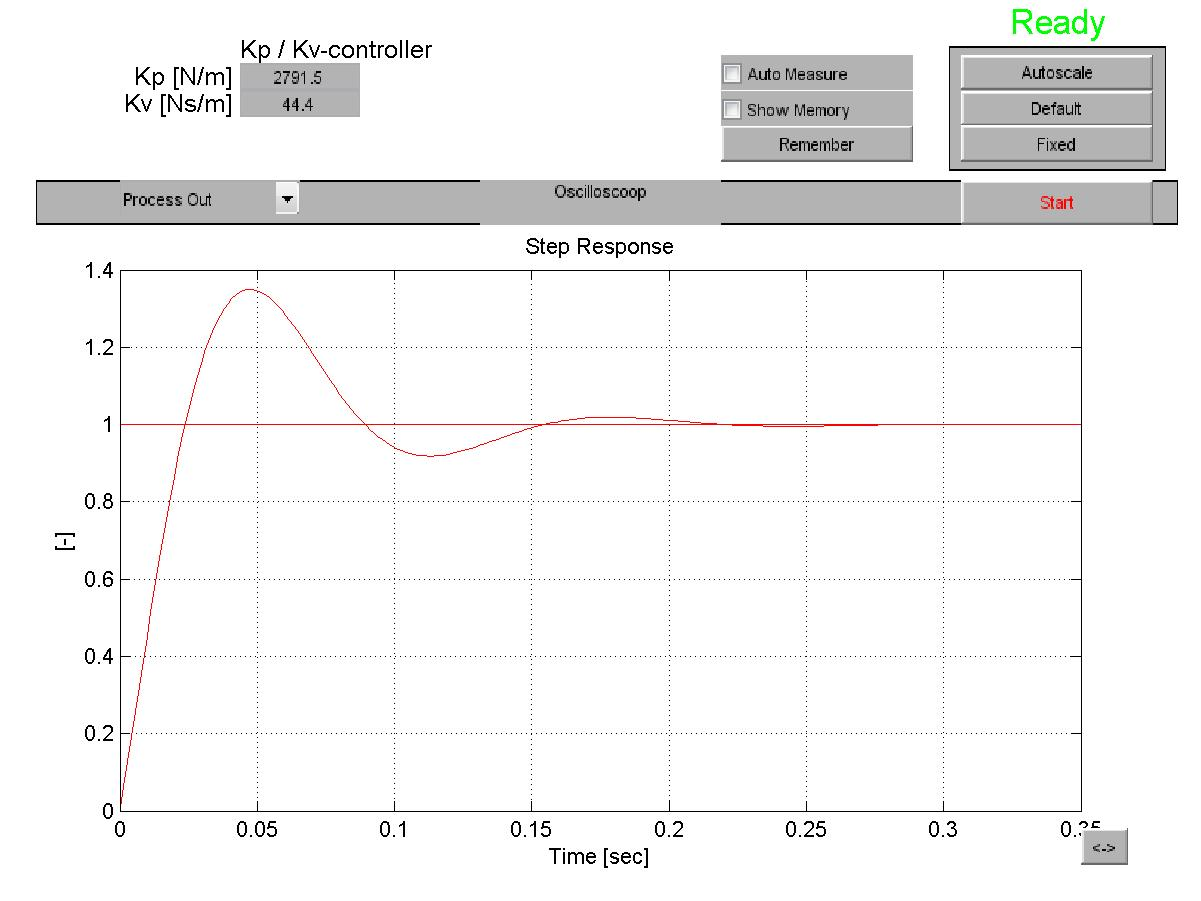
\includegraphics[width=\textwidth,height=\textheight,keepaspectratio]{1A6_bw_10}
\caption{Step response plot of the single mass system with controller $C(S)$ tuned for bandwidth $10 Hz$ and phase margin $45\deg$}
\label{fig:1A6_bw_10}
\end{figure}

When the bandwidth is increased and the following parameters are used: 
\begin{itemize}
\item{$bw = 10 Hz$}
\item{$PM = 45\deg$}
\end{itemize}
This results in the step response plot in figure ~\ref{fig:1A7_bw_50}
\begin{figure}
  \centering
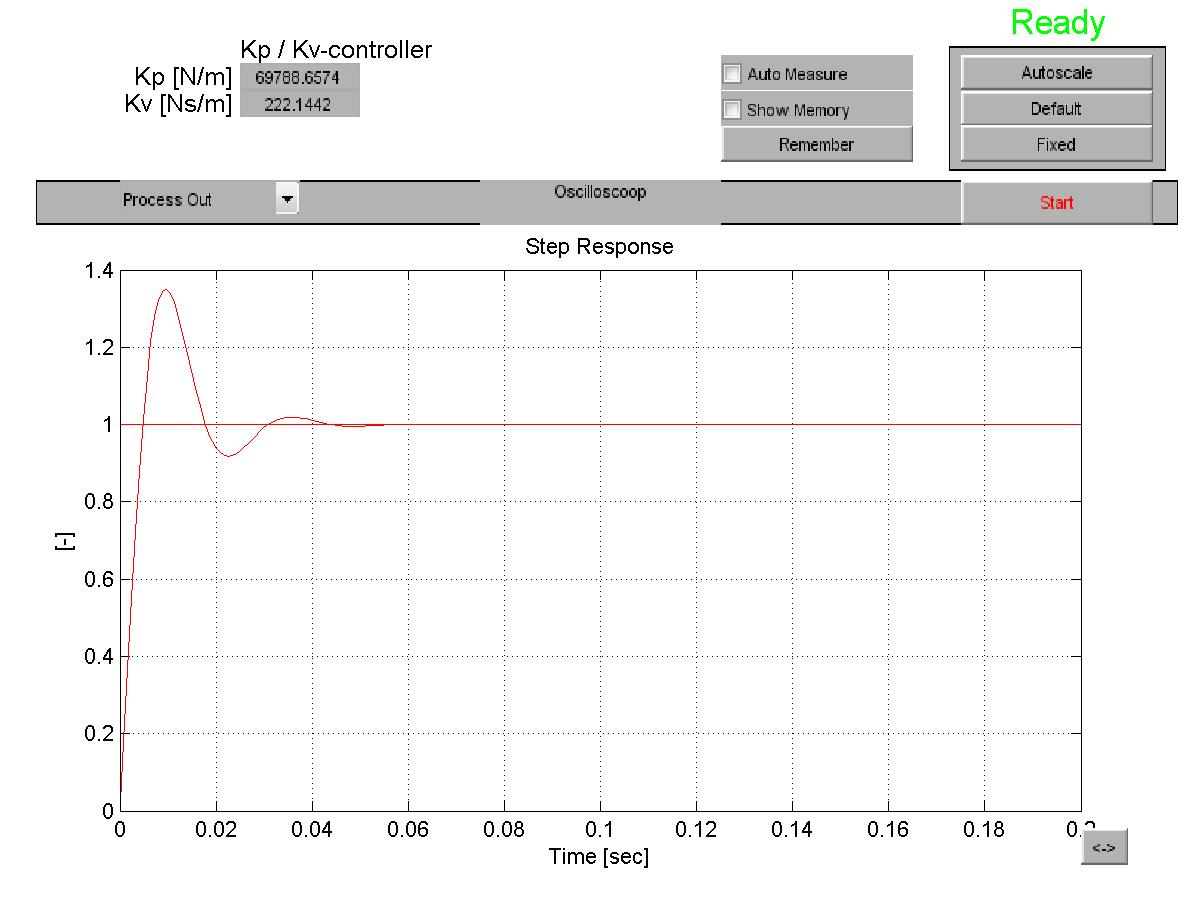
\includegraphics[width=\textwidth,height=\textheight,keepaspectratio]{1A7_bw_50}
\caption{Step response plot of the single mass system with controller $C(S)$ tuned for bandwidth $50 Hz$ and phase margin $45\deg$}
\label{fig:1A7_bw_50}
\end{figure}

Evaluating the controllers with the different bandwidth gives some similarities. 
First of all they both have a overshoot near $35$ percent and a little oscillation afterwards. Also there is no steady state error. 
The biggest difference is the rise time and settling time of the controllers. The controller with the bandwidth of $50Hz$ is much faster than the one with the $10Hz$ bandwidth.  

%Effecten:

%Zero verplaatst naar hogere frequenties bij hogere k_p

%Kp verhoogt de totale gain van bij verhoging
%Kv verplaatst de zero richting de lagere frequenties
%Tegelijkertijd wordt ook de cross over frequentie 
\end{document}





